\documentclass[%
  chapterprefix=false,%
  open=right,%
  twoside=true,%
  paper=a4,%
  logofile={Figures/logo.png},%
  thesistype=master,%
  UKenglish,%
]{se2thesis}
\listfiles
\usepackage[ngerman,main=UKenglish]{babel}
\usepackage{blindtext}
\usepackage[%
  csquotes=true,%
  booktabs=true,%
  siunitx=true,%
  minted=true,%
  selnolig=true,%
  widowcontrol=false,%
  microtype=true,%
  biblatex=true,%
  cleveref=true,%
]{se2packages}

\addbibresource{ref.bib}

\usepackage{hyperref}
\usepackage[caption=false]{subfig}

\author{Gonzalo A. Oberreuter Álvarez}
\title{Master Thesis Proposal}
\degreeprogramme{Computer Science}
\matrnumber{110082}
\supervisor{Prof.\,Dr.~Gordon Fraser}
\external{}
\advisor{}
\department{Faculty of Mathematics and Informatics}
\institute{Chair of Software Engineering}
\location{Passau}

\begin{document}

\frontmatter

\maketitle

\iffalse{}

\authorshipDeclaration{}

\begin{abstract}
  An English abstract to the thesis. 
  TBD.\@
\end{abstract}

\begin{abstract}[german]
  Eine deutschsprachige Zusammenfassung der Arbeit.
  TBD.\@
\end{abstract}

\begin{acknowledgements}
  Some acknowledgements. 
  TBD.\@
\end{acknowledgements}

\tableofcontents

\fi

\mainmatter{}

\chapter{Introduction}

Software Testing is one of the key aspects of Software Developing while trying to ensure quality over a final product, regardless of the context in which the developing process is made.
This quality can be achieved by the insight provided by the result of the tests, and even because of the defects that can be encountered during the testing phase.
Nonetheless, even though coding different kinds of tests is a good practice, it is often ignored by new or inexpert developers, who also make this mistake halfway by not getting a complete introspection of their own code or, in other words, not getting a complete kind of test coverage.
As of 2017, a study by Trauch and Grabowski~\cite{DBLP:conf/icst/TrautschG17} presented that, over more than 4 million tests, most of them weren't correctly categorized (as unit test or not) and approximately half of them use mocking as a testing technique, which tells some aspects about the developing community of the projects in review. 
With this general idea into mind, is that researchers in the last decade   have put effort into autonomous test generation, the concept that implies the usage of different methods or techniques in order to identify patterns and generate test sets with little to zero   external intervention.
In 2015, empirical proof was found who showed the following statements about the usage of automated Java unit test generation:
\begin{itemize}
  \item It increases the general structural coverage
  \item It does not lead to the detection of more faults
  \item It affects negatively the ability to capture intended class behaviour
\end{itemize}
according to Fraser et al.~\cite{DBLP:journals/tosem/FraserSMAP15}
The results of this study state fundamentally that this behaviour  comes from the early stages of the tool in question, and proposes to put more work into the readability of generated tests and  the process of test making itself.

Although automatic test generation is achievable with no major problem for statically typed languages like Java~\cite{DBLP:journals/tse/FraserA13} or C, dynamically typed languages such as Python, JavaScript or Lua enforce problems at the time of generating correct parameters for the execution of methods or function under test.
%Explain what a dynamically typed language is?
The major concern about the parameter generation, is that the lack of type information produces ambiguity for the heuristics of the tool at hand at the moment of synthesizing non-primitive types.
Also, the complexity of this object or callable types might produce runtime errors, which imply a local optima in the search landscape of the test representation~\cite{DBLP:conf/sigsoft/0001O00D21} and therefore an upper bound for coverage.

Within the scope of Python testing, Pynguin~\cite{DBLP:conf/icse/LukasczykF22} is a test generation framework that applies various algorithms for input generation, such as DynaMOSA~\cite{DBLP:journals/tse/PanichellaKT18}, MIO~\cite{DBLP:conf/ssbse/Arcuri17}, MOSA~\cite{DBLP:conf/icst/PanichellaKT15}, random~\cite{DBLP:conf/icse/PachecoLEB07}, Whole Suite~\cite{DBLP:journals/tse/FraserA13}, and Whole Suite with archive~\cite{DBLP:journals/ese/RojasVAF17}.

\begin{figure}[tb]
  \centering
  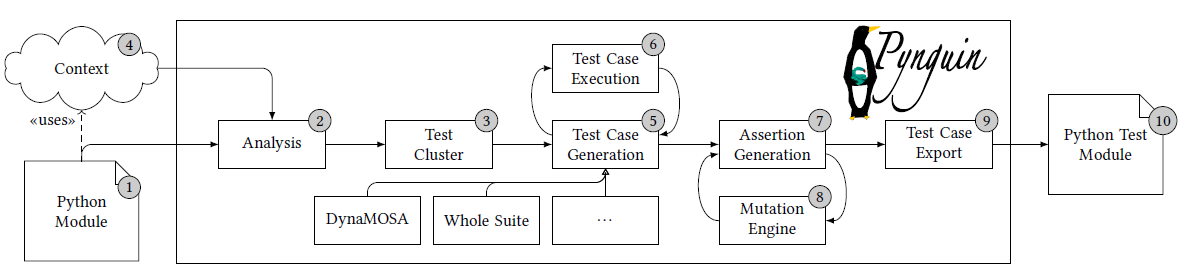
\includegraphics[width=.99\textwidth]{Figures/pynguin.png}
  \caption{Pynguin structure}\label{fig:pyn}
\end{figure}

Its structure is presented in Figure~\ref{fig:pyn} and consists of 10 autonomous steps that work in the following manner
\begin{enumerate}
  \item The unit test generation process starts with the input of a user defined python module that needs to be tested.
  \item The module is then analysed in order to obtain primordial information, such as all the functions, classes and their respective attributes and methods, together with their respective parameters.
  \item In the Test Cluster, all the information gathered from the analysis of the module under test (MUT) and its relevant dependencies.
  \item As mentioned in the previous item, the Context step performs an inter procedural analysis of all the libraries and modules used by the actual MUT, and joins any new obtained information with the data in the Test Cluster.
  \item The Test Case Generation step, individually picks functions or methods from the Test Cluster in order to generate the internal representation, firstly by creating a statement using the function or method in question, and then generating an argument for every parameter.
  \item After a Test Case Generation is performed, it is executed to get the desired coverage and analyse if (a) it already reacher the maximum or (b) a new better Test Case should be generated.
  \item Once the stopping conditions are met, the test cases are finished with an optional assertion to check the results of the testing.
  \item Alternatively, mutations of the test cases are created using MutPY, so Pynguin can evaluate if the previously created assertion kill or not the mutants.
  If they do not, new assertions are created.
  \item In the Export step, Pynguin translates the test cases from its internal representation into test code with the format of the library PyTest.
  \item Finally, these tests are written into a final module.
  
\end{enumerate}
%Is this plagio?
At the time of its original release (25th of July 2020), Pynguin was a state-of-the-art open source tool that has made the first step for subsequent researches about how to improve the performance and functionalities of Pynguin itself, including CodaMOSA~\cite{DBLP:conf/icse/LemieuxILS23}, PyLC~\cite{DBLP:conf/sac/SalariEAS23} and many other tools that will be briefly explained in the State of the Art section.

These recent new extensions of Pynguin and the aforementioned problem at the time of generating complex object inputs are the principal motivations of this thesis and the related and future work to it.

\chapter{Proposal}

The original Pynguin research paper~\cite{DBLP:conf/icse/LukasczykF22} stated that after the test generation of 118 Python modules, the average branch coverage over all algorithms was $66.8\%$, which leads to think that improvement is possible.

%talk about how coverage isn't everything?
The current Master's thesis proposes an addition to the original structure of Pynguin~(see~Figure~\ref{fig:pyn}), specifically to sections (5) and (2) by developing a Graph-Based Object Synthesis approach~\cite{DBLP:conf/sigsoft/0001O00D21} (GBOS) and the usage of a type information modifier module respectively, in order to diminish the branch coverage gap, try to generate more complex test suites and empirically study the effect of the presence of type information.

\begin{figure}
    \inputminted[linenos]{python}{Figures/example.py}
    \caption{Module example.py\label{lst:1}}
\end{figure}

\begin{figure}
  \inputminted[linenos]{python}{Figures/dependencies.py}
  \caption{Dependency module of example.py\label{lst:2}}
\end{figure}

As an example, Listings~\ref{lst:1}~and~\ref{lst:2} represent a MUT and its dependency module, respectively, in which lines 8, 10 and 12 of the MUT are the targets of the branch coverage problem.
Even though the test suite generated by Pynguin (see Listing~\ref{lst:3}) gets to a branch coverage of \(\%37.5\) (using DynaMOSA, the seed 1998 and 100 seconds as stopping condition), it can be inferred that this result comes from \verb|test_case_1()|, that executes one of the first two branches in MUT and check if the variables \verb|actor| and \verb|target| are actual \verb|Player| objects.
This behaviour prevents Pynguin from escaping the local optima.
At this point, the idea of using a graph for the synthesis of objects is to get Pynguin to generate a \verb|GameState| object with the necessary \verb|Players| in the \verb|players| list, and a \verb|Action| object with correct attributes, so a hypothetical test could reach the third branch in the MUT, even if it is with a false guard.
  
\begin{figure}
    \inputminted[linenos]{python}{Figures/test1.py}
    \caption{Test suite generated by Pynguin for module example.py\label{lst:3}}
\end{figure}

The Graph-Based heuristic proposed by Lin et al.~\cite{DBLP:conf/sigsoft/0001O00D21} generates an object construction graph (OCG) from a previous code slicing, performed from the program dependency graph and a specific target branch as criteria.
This branch must be selected from those who have not reached their full coverage, or are ``non-trivial'', and the depth of the intra procedural dependency should be set as an arbitrary level $t_{\text{dep}}$.
Then, this OCG is used to generate a code template that should be either translated directly into the test code representation of Pynguin or an intermediate form.
Pynguin, similarly to other search-based test generating tools, represents its test cases as a sequence of implementations of a super class \textit{Statement} that can be later transformed into an Abstract Syntax Tree and an actual block of Python code.
This previous idea was completely implemented in and for Java, which means that part of the work to be done is to ideate a new Python representations of the OCG.\@
Listing~\ref{lst:4} shows the code of a statement sequence template for the testing of the example module that still gets a run time error in line 18.
However, this template allows Pynguin to get out of the local optima, if right values are modified in the correct variables.

\begin{figure}
  \inputminted[linenos]{python}{Figures/template.py}
  \caption{Potential test template obtained through the use of an OCG\label{lst:4}}
\end{figure}

The usage of a type information modifier library is mentioned, because it will be applied in order to review how the general type information of a Python project affects in the ability of the GBOS approach to generate correct object inputs templates.
The reason for this is, as stated before, Python being a dynamically typed language and not requiring the type of variables in the script in order to be executed.
To illustrate this, if line 4 in Listing~\ref{lst:1} were to be replaced to \mint{python}|def checkRules(self, action, state) -> bool:| it would make Pynguin not have any information about the type of the parameters, and generate a test suite similar to the one in Listing\ref{lst:5}.
The behaviour that allows Pynguin to generate the previous suit imply that the current type system implemented as part of Pynguin does not work properly when trying to infer object types.

\begin{figure}
  \inputminted[linenos]{python}{Figures/test2.py}
  \caption{Test suite generated by Pynguin for a variation of module example.py\label{lst:5}}
\end{figure}

After the implementation part is done, a study of the extension will be made through the selection of arbitrary sets of Python modules, being these either the original research paper's or a new set that ensures the explicit type of object inputs and a ratio of this kind of inputs of more than $50\%$.
The final purpose of the thesis is to obtain a Cohen's d effect size over the coverage results between Pynguin and the proposed extension, and compare it to the ones obtained between EvoSuite and EvoObj.
A further analysis of the difference in this metric shall also be done.

The previous setup can be structured by the following research questions and further explained by their experimental implications:

\resq{Can the Graph-Based Object Synthesis extension outperform Pynguin in its original paper's experimental setup similarly as EvoObj did with EvoSuite?}

For the answer of this Research Question, the archive of the projects used for the experimental setup of Pynguin in its release paper\footnote{https://zenodo.org/records/6838658} will be put again to the test to benchmark the performances of both Pynguin in its latest version (0.25.0) and the extension to the tool to be presented by this thesis.
While trying to follow a similar configuration to the one presented in all the papers featuring Pynguin, all the algorithms available in the latest version will be executed with their default settings, and 30 times per module.

\resq{How is the performance of the GBOS extension with respect to Pynguin in a context where the MUT have mainly objects as inputs?}

To generate the adequate context, the same Test Cluster of Pynguin can be used as a way to acknowledge modules that actually have objects (different to the built-in objects, such as Lists, Tuples, Dictionaries, etc) as part of the signature of its methods, functions or constructors.
Taking advantage of this feature, the experimental modules can be filtered and gathered in order to accumulate a set of libraries that largely have objects as input types rather than primitive or other built-in types.
In addition, all trivial modules that get full branch coverage in first stages of the search-based algorithm used for filter (most likely DynaMOSA, in either under 10 seconds or 10 iterations) will also be filtered. 

\resq{What is the impact of the presence of parameter type information in the automatic generation of tests by the GBOS extension?}

This last research question essentially makes room for two kinds of MUT:\@
\begin{itemize}
  \item those who originally do not have type information in their functions' signatures and should be inferred by using any possible mean to improve the coverage and, 
  \item those that do have their respective type information and should lose it to check the impact of this loss.
\end{itemize}

These two sets of MUT can be obtained directly from the MUT from the previous research question, making a partition between the filtered and non filtered ones.
If a suitable type inference library can be found, the first set of modules will be used for the research of this question while adding to them the respective type information, and the second set will be used in the contrary case.


\chapter{State of the Art}

%\textbf{If the state-of-the-art papers mention different kinds of tests (unit, regression, etc), maybe its a good idea to explain them.}
%\textbf{Also, some other concepts should be stated, such as acronyms for subject under test for generalization.}

\section{EvoSuite}

With respect to Unit Test Generation, EvoSuite~\cite{DBLP:conf/qsic/FraserA11} was (and still is) a state-of-the-art test generation tool for Java, pioneer of the usage of a genetic algorithm, so the branch coverage can be optimized as a whole.
The internal representation of EvoSuite for a test suite is a set of \textit{chromosomes} \(T\) as a sequence of statements \(t_i\) of length \(l_i\) and either type primitive statement, constructor statement, field statement, or method statement.
During the chromosome synthesis process, all the information regarding classes, methods and variables of the SUT are gathered via the Java Bytecode and Java Reflection\footnote{https://docs.oracle.com/javase/8/docs/technotes/guides/reflection/index.html}.
These sequences can be crossovered as a random sequential combination of the two \textit{chromosomes}, or mutated with the insertion, remotion or change of single statements.
In terms of the optimization, the fitness function of a test suite $T$ is given by the equation
\[ \text{fitness}(T) = |M| - |M_T| + \sum_{b_k \in B} d(b_k, T) \]
where $M$ is the total of methods to test, \(M_T\) is the number of methods that were actually executed, \(b_k\) is a branch in the branch set \(B\), and \(d(b, T)\) is the branch distance of branch \(b\) over the set \(T\).
Another limitation to the suites \(T\), are \(N\) as the maximum number of chromosomes (\(T = \{t_1, \dots , t_n\}\)) and \(L\) as maximum length of the chromosomes (\(l_i < L\)).
For the experiment phase, a single branch approach was created by the authors, in which every branch \(b_t\) is seen as a single coverage goal to be met by the test cases.
Then, the comparison between the single branch method and the whole suite optimization is done with the generation of test cases for five open source projects, accumulating a total of 1308 classes from which 727 were public.
After the execution of test cases was complete and statistical tests were applied, it could be stated that the results show EvoSuite has a better branch coverage and creates smaller tests suites than the single objective method.

\section{NxtUnit}

\begin{figure}[bt]
  \centering
  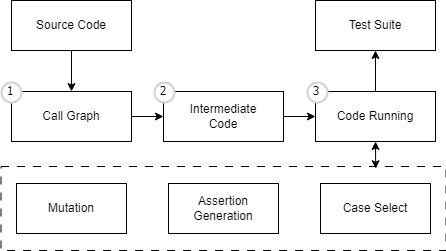
\includegraphics[width=.99\textwidth]{Figures/nxtunit2.png}
  \caption{NxtUnit structure}\label{fig:nxt}
\end{figure}

Having EvoSuite, Randoop and Pynguin as precedents, in 2023 developers from ByteDance (technology Chinese company) presented NxtUnit~\cite{DBLP:conf/ease/WangMCGSP23}, an automatic randomized test generation tool for the programming language Go.
Similar to other state-of-the-art tools, the structure of NxtUnit (see Figure~\ref{fig:nxt}) is composed by an initial source code as input, that is translated into Static Single Assignment form as a way to get a graph with call dependencies between functions.
After this preprocessing, NxtUnit proceeds to synthesize from the call graph a code template that will be filled with appropriate randomly generated parameters and ran during the tool's execution.
All the information for the template synthesis and posterior parameter changes will be done thanks to the information provided by Go Reflect\footnote{https://pkg.go.dev/reflect}.
During the code running phase, NxtUnit focuses in three main tasks: mutation of the parameter inputs at runtime, assertion generation for future regression testing, and test case selection based on code coverage.
Once the tool comes to a halt, the best test cases are exported into a test suite.
In the experiment proposed by the authors, NxtUnit was executed on 500 private ByteDance repositories and 13 out of the 100 highly-rated public repositories of Go, both sets that already contain tests.
The main objective of this setup, was to review the code coverage increase while adding NxtUnit tests to the already existing ones, and it produced an average increase of \(5.51\%\) for the public repositories and \(17.26\%\) for the private ones.

\section{JSEFT}

As an example for automatic test generation in dynamic languages others than Python, JSEFT is presented in 2015 by Mirshokraie et al.~\cite{DBLP:conf/icst/Mirshokraie0P15} as a tool for generating not only unit tests, but also event-driven tests for web applications written in JavaScript.
The general structure of JSEFT is presented in Figure~\ref{fig:jseft} and is composed of three main steps that process the data given by the HTML Document Object Model (DOM):
\begin{itemize}
  \item In (1) the web app is dynamically analysed in order to get all the possible states of the program and, in consequence, construct a state flow graph (SFG)
  \item Then, in step (2), event sequences are extracted from the SFG for the creation of event-driven tests, which will be run in the instrumentalized version of the web app.
  With these executions, JSEFT tries to discover DOM states and entry and exit state points for the creation of function-level unit tests
  \item Finally, the third step (3) mutates the web app at code and DOM level, so functional oracles can be created from the difference between the two states of the original and mutated tests versions
\end{itemize}

\begin{figure}[tb]
  \centering 
  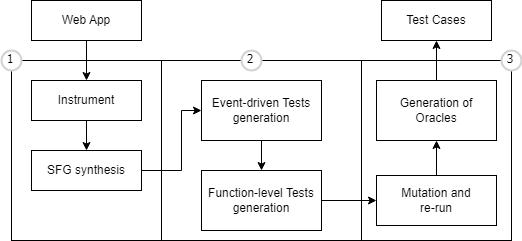
\includegraphics[width=.99\textwidth]{Figures/jseft2.png}
  \caption{JSEFT structure}\label{fig:jseft}
\end{figure}

For the export of event-driven and function-level tests, the frameworks Selenium\footnote{https://www.selenium.dev} and QUnit\footnote{https://qunitjs.com} are used respectively.

The experiment section of the author's paper, shows the study of JSEFT's usage on 13 JavaScript web applications so the line coverage and usefulness of the assertions at the time of finding regression faults.
For the specified metrics, the tool got a \(68.4\%\) of line coverage and a \(100\%\) precision in fault detection.

%\section{LUTG}

\section{CodaMOSA}

One of the many tools presented in papers that have cited Pynguin in their research is CodaMOSA~\cite{DBLP:conf/icse/LemieuxILS23}, software created by Microsoft developers, has Pynguin as a base and extends its functionality calling OpenAI's Codex\footnote{https://openai.com/blog/openai-codex} API to get template suggestions for test cases that are in a coverage stall, similar to what this thesis works over.
For the development, the authors used only MOSA as the search algorithm because is the only one that allowed the usage of both line and branch coverage as fitness functions, on the version of Pynguin at the time (0.19.0).

The procedure done by CodaMOSA, queries prompts to Codex after the coverage has not changed in a certain amount of iterations, and from a set of target generations of chromosomes that it statistically chooses to generate a test from either a function, method or constructor.
After that, it deserializes the returned test case from Codex into the internal representation of Pynguin, while applying different heuristics, such as removing nested expressions and use single assignment.

For the benchmark, modules from 35 projects from the Pynguin paper were filtered so just those that do not fail to produce result and those that do not reach \(100\%\) coverage in less than a minute are experimented over.
The baselines for the experimental phase were Pynguin with MOSA and CodexOnly, which while being compared to CodaMOSA were statistically compared using the Mann-Whitney U-Test.
The results showed that CodaMOSA performs significantly better, reaching a higher coverage on 173 more modules compared to MOSA and 279 more modules compared to CodexOnly.

\section{PBT-GPT}

Property-based testing (PBT) is a kind of fuzz testing whose idea is to generate a large amount of random inputs to statistically test a program by checking if the outputs are close to a desired property.
Within this scope, PBT-GPT~\cite{DBLP:journals/corr/abs-2307-04346} is presented by Vikram et al.\ as an implementation of automatic property-based test generation for Python by means of Large Language Model prompting, through Chat-GPT4.
The general idea of this testing approach, is to operate with three different prompting approaches to generate Python tests of specific module methods while using \textit{Hypothesis}\footnote{https://hypothesis.readthedocs.io/en/latest/}, a PBT library specialized in input generators, and the API documentation of the so-called method.
These three strategies for prompt calling are named and described as the following

\begin{itemize}
  \item Independently, where both the prompts for the input generator and properties assertion are synthesized from independent instances of Chat-GPT, and then combined in a single Python code snippet
  \item Consecutively, where the prompts are executed sequentially on the same instance of the LLM and combined at the end
  \item Together, where all necessary prompts are combined, and called singularly in an instance of LLM
\end{itemize}

and have as context for the prompt, the LLM being an expert in Python, the LLM needing to review the API documentation, instruction to generate a PBT component, and the desired output format.

For the result evaluation quality, the authors were guided by; generator validity and diversity, that measure either the correct behaviour or diversity of inputs; and property validity, soundness and strength, that measure the encounter of runtime errors, the existence of input/output pairs that violates the property but is valid at the same time, or the ability to check core logic of an API method.
With these guidelines, the modules/methods under test got measurements close to \(100\%\) in generator validity and property validity, and between \(68\%\) and \(88\%\) for the rest of them, which helps conclude that PBT-GPT is a promising starting point to iterate from.

\section{CodeT}

Following the examples of software artefacts presented by Microsoft developers, in 2022 is published a paper regarding CodeT~\cite{DBLP:journals/corr/abs-2207-10397}, a LLM based code generation tool.
The main purpose of CodeT is the solution of a programming problem by generating a code snippet, based on a context containing natural language.
Regardless of this not being in the same direction of the previous software examples, test generation using the same LLM is part of the whole process, although all of these just have the form of a single assertion, together with a set of inputs and the desired output.

\begin{figure}[tb]
  \centering 
  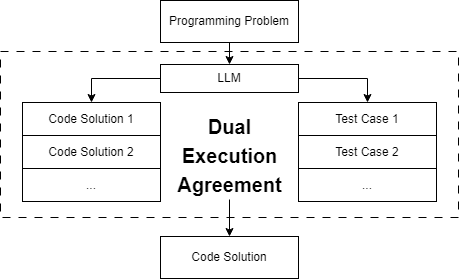
\includegraphics[width=.99\textwidth]{Figures/codet.png}
  \caption{CodeT structure}\label{fig:codet}
\end{figure}

A general structure of CodeT is shown in Figure~\ref{fig:codet}, which also depicts the functioning of it by first, prompting the generation of a set of tests (right on the figure) based on the natural language context of the programming problem, that will later be at the same time the context for the prompting of a set of code snippets (left on the figure).
After the execution of the LLM model is finished and all the outputs are gathered, a \textit{Dual execution agreement} criterion, based on the RANSAC~\cite{DBLP:journals/cacm/FischlerB81} algorithm, is used to select the best code solution.
The selection in this criterion, is done by forming consensus sets of both code solutions and test cases, by selection a valid pair \((x_\text{code}, y_\text{test})\) as a hypothetical inlier, and grouping it with all tests that are also passed by \(x_\text{code}\) in set \(S_y\) and all other code snippets that pass the same tests as \(x_\text{code}\) in set \(S_x\).
Finally, when all consensus sets \(S_x\) and \(S_y\) are formed from the different valid pairs \((x_\text{code}, y_\text{test})\), those with the highest cardinality \(f(S) = |S_x||S_y|\) will have the best score for selection.

As stated before, CodeT centres around code generation rather than test case generations, which makes the research of this paper focus mainly on metrics such as pass@1 or pass@100 (correct rate of single solutions, or at least one for every hundred).
Nonetheless, to check the quality of the generated solutions, the authors also covered in their result analysis the code and branch coverage of the snippets generated from the different LLM models.
Almost all the models obtained an overall average coverage of \(95\%\).

\section{MutAP}

Mutation testing is one software testing technique, that aims to measure the ability of a test to reveal bugs.
Taking this approach in mind, Dakhel et al.\@ presented in 2023 MutAP~\cite{DBLP:journals/corr/abs-2308-16557}, another LLM based code generation tool that also introduces prompt augmentation for killing mutants in an iterative process before the actual synthesis of test cases.

\begin{figure}[tb]
  \centering 
  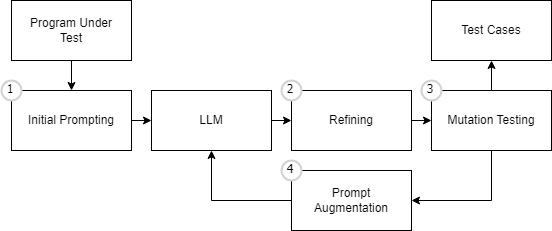
\includegraphics[width=.99\textwidth]{Figures/mutap.png}
  \caption{MutAP structure}\label{fig:mutap}
\end{figure}

A summary of MutAP's structure is shown in Figure~\ref{fig:mutap}, and after inputting a Python Program Under Test (PUT), it commences with the building of an initial prompt for the obtaining of an initial test case.
The first step (1), employs one of the two following learning methods; zero-shot, where the PUT is concatenated after the statement  ``Generate test case for the following code''; and few-shot, which concatenates the PUT after a sequence of pairs of a method and its respective unit test.
After the initial test is synthesized, the second step (2) consists of re-prompting it, so possible syntax errors can be corrected and unintended behaviour can be repaired.
Then, the third step (3) introduces mutations into the PUT using MutPy\footnote{https://pypi.org/project/MutPy/0.3.0/} so that the quality and effectiveness of the tests can be assessed.
At this point, the algorithm of MutAP has a conditional path depending on the number of surviving mutants; if there are none, the test cases are considered finished and generated; and in the contrary case, the prompt augmentation step is followed.
This post conditional step (4), adds information to a new prompt of the LLM, such as the already refined initial test, the statement ``The test function, test(), cannot detect the fault in the
following code'', one of the mutant survivors, and a final statement ``Provide a new test case to detect the fault in prior code''.

In the experimental trial of this tool's paper, two LLM models were used, OpenAI's Codex and llama2-chat, to be run together with MutAP over the benchmarks; HumanEval, which consists of 164 human written programming problems; and Refactory, consisting of 1710 buggy submissions from students for 5 assignments of a Python programming course.
The overall results mainly cover the mutation score obtained by all the possibles methods of MutAP, obtaining numbers between \(89.13\%\) and \(93.57\%\) on the average over both models and both datasets.

\section{MUTester}

MUTester~\cite{DBLP:journals/corr/abs-2307-00404} is an automatic test generation research software focused on the synthesis of test cases for APIs of the many already existing Deep Learning libraries, i.e. Numpy, Scikit-learn, TensorFlow.
Its structure is presented in Figure~\ref{fig:mutester}, which describes a methodology that solely relies on heuristics regarding the mining of the documentation and knowledge repositories of the APIs in question. 

\begin{figure}[tb]
  \centering 
  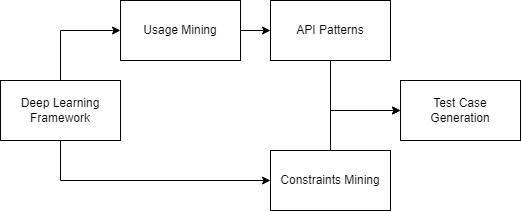
\includegraphics[width=.99\textwidth]{Figures/mutester.png}
  \caption{MUTester structure TODO: Add numbers}\label{fig:mutester}
\end{figure}

The first half of the repository mining (1) is done by applying web scrapping to the documentation pages of the different methods of the libraries, so that information regarding input type (via signature definition mining) and constraints can be gathered, which as mentioned before, is crucial for a correct test generation.
Input constraints are collected from the natural language parameter description that is usually presented in Python documentation pages, and rather than extracted using a LLM model, they are identified using by recognizing linguistic patterns.
A last piece of information that is gathered in this step are any code snippet example, so any useful input can be statically analysed.

Stack Overflow is the source of information for the second half of repository mining (2), from where the authors extracted from any related (question, accepted answer) pair the code snippets that had relevant method sequences in them.
Then (3), these method call sequences are studied using the Apriori~algorithm~\cite{agrawal1994fast} to look for intrinsic rules between the calls.

Finally, test case generation (4) is managed as a guided synthesis of a call sequence, that ends in the actual method under test, similar to what Pynguin does, but with the help of all the relationship information obtained in the previous steps.
Similarly, the input generation is conducted.

Throughout the analysis of MUTester, the API documentation and methods of the frameworks,  Scikit-learn, PyTorch, TensorFlow and CNTK were accounted for.
Regarding test coverage, the baselines for the experimentation were Pynguin and a Python implementation of Randoop, which achieved \(34.16\%\) and \(30.87\%\) line coverage in average, versus the results obtained by MUTester, that showed improvements ranging from \(15.72\%\) to \(27\%\).
A Wilcoxon signed-rank
statistical test~\cite{Rey2011} was also applied to the results, obtaining a p-value of less than \(0.05\) suggesting that MUTester outperformed both baselines in the stated datasets.


\iffalse{}
\begin{itemize}
  \item State of the unit test generation in python
  \begin{itemize}
    \item LExecutor~\cite{DBLP:journals/corr/abs-2302-02343}
    \item ChatGPT~\cite{li2023nuances}
    \item PyLC~\cite{DBLP:conf/sac/SalariEAS23}
  \end{itemize}
\end{itemize}

Comments on the state of the art
\fi

\backmatter{}

\printbibliography{}

\end{document}
